\documentclass[12pt, oneside]{article}   	% use "amsart" instead of "article" for AMSLaTeX format
\usepackage[margin=1in]{geometry}                		% See geometry.pdf to learn the layout options. There are lots.
\geometry{letterpaper}                   		% ... or a4paper or a5paper or ... 
%\geometry{landscape}                		% Activate for for rotated page geometry
%\usepackage[parfill]{parskip}    		% Activate to begin paragraphs with an empty line rather than an indent
\usepackage{float}
\usepackage{graphicx}				% Use pdf, png, jpg, or eps§ with pdflatex; use eps in DVI mode
%\usepackage{amsmath}
%\usepackage{CJK}	% convert eps --> pdf in pdflatex		
\usepackage{achemso}
\usepackage{amssymb}
\usepackage{indentfirst}
\usepackage{url}


\title{Predicting Chemical Properties Using Machine Learning Methods}
\author{Andrew IDs: ccollin1, haichenl, zhonghal}
%\date{}							% Activate to display a given date or no date

\begin{document}
\maketitle

\begin{abstract}
To be filled.    
\end{abstract}
\section{Introduction}
%\subsection{}
\noindent Quantum mechanics allows us to predict chemical compounds' properties to a very high accuracy, given that we are able to solve certain nonlinear ill-conditioned partial differential equations. Density Functional Theory (DFT) and \textit{ab initio} theory are two common types of methods to solve quantum differential equations; they possess the powerful advantage that in principle they are applicable to every type of chemical compounds. DFT has been used extensively for predicting chemical properties as a proper compromise between accurate (yet extremely expensive, typically $O(n^7)$ to $O(n!)$ in both time and space) \textit{ab initio} methods and cheap ($O(n^2)$ but can only achieve qualitative accuracy) Semi-Empirical Quantum Chemistry (SEQC) methods. Unfortunately, DFT methods still scale at least as $O(n^4)$ in both time and space, which means that they can only be applied to chemicals that have on the order of hundreds of atoms. Unfortunately, often in chemistry research, people deal with chemicals that consist of thousands of atoms every day (or hundreds of thousands in the case of biochemistry). The main benefit of a machine learning approach to doing these calculations would be that it could potentially be much faster and still retain the same level of accuracy as slower DFT calculations.

Recent studies show that a variety of machine learning regression models can be employed to predict chemical properties. Instead of solving partial differential equations directly, machine learning models try to predict chemical properties from "chemical similarities". From a chemist's point of view, chemicals are made of only a small set of structural building blocks, the properties of which have been thoroughly studied. Molecules consisted of similar building blocks are very likely to share similar chemical properties. Therefore, it is reasonable to train our machine learning models with features come from chemicals made of only a few building blocks, then use these models to predict properties of chemicals that constitute a great number of building blocks. An analogy is to train a spam filter with e-mails that have only a few sentences, and hope that this filter can classify not only short e-mails but also long e-mails that have similar sentences as our training examples do. Unlike quantum mechanical models which are considered "universal", our models will be, for sure, only applicable to a subset of chemicals, but that is just the inevitable trade-off between accuracy and generality. \\

Philosophically, our feature engineering part is highly related with our chemistry knowledge about our target molecules. It is expected that we can extract chemically informative characteristics of every molecule in both training stage and test stage. We have implemented 6 different ways to transform structural features of all the sample molecules into feature vectors. On the other hand, our training labels are supposed to be generated through quantum mechanical calculations, which require a solid understanding of the physics behind. Right now we basically treat this type of calculation as a black box, but in quantum chemistry there exist ways about how to reformulate complicated partial differential equations into simple ones--that is what most of the SEQC methods do, and we are planning to take advantage of this point in feature engineering. Specifically, we are interested in establishing regression models of the energies of highest occupied molecular orbital (HOMO), lowest unoccupied molecular orbital (LUMO), and band gap. These 3 properties are of great chemistry/physics interests both theoretically and experimentally, since they are directly related with molecules' spectroscopic behaviors. Our goal is to predict these chemical properties with machine learning methods that are cheaper, and produce ``chemical accuracy" (1 kcal/mol (0.047 eV)).\\

In this report, several common polymer chains are constructed as samples and their HOMO, LUMO and band gap are calculated as labels. We develop 9 different types of feature vectors to employ supervised machine learning methods, including Linear Regression, Linear Ridge Regression, Support Vector Machines (SVM), K-Nearest Neighbors (k-NN), Decision Tree, Boosting and Neural Networks. Details on dataset construction, feature engineering, methodology and model developments are demonstrated in the following sections. We will also present corresponding training/testing errors of combinations of different feature vectors and machine learning models later in this report. \\

\section{Data and Feature Vectors}


\noindent Right now we have 1500 characteristic polymeric systems (chemicals that are built from repeated units, like plastic/rubber/Nylon) in our tentative training set. These systems are made up from 7 different major building blocks, (phenyl, furan, vinyl, acetylene, pyrrole, pyridine, and ketone), and 7 minor building blocks, (Hydrogen, methyl, hydroxyl, methoxy, carbenyl, cyano, and amine). Some visualized polymer structures are shown in Fig ~\ref{furan}. They are divided into one group that consists of Oxygen (O) and another group that consists of Nitrogen (N) for chemical analysis. Quantum chemistry software package \textit{Gaussian} \cite{gaussian} is applied to compute HOMO, LUMO and band gap at three different DFT levels, namely B3LYP, CAM-B3LYP, and M06HF. Fig ~\ref{orbital} shows the an example calculated HOMO and LUMO. These 3 theories have been widely tested in chemical research, and they lead to slightly different numerical results. In addition, each of these methods defines an energetically favored geometrical structure for each of the molecules; these structures are slightly different, and it is reasonable to think that each of them contains some information. Along with the initial non-optimized geometrical structure, we have 4 types of structures; combining with the aforementioned 3 DFT theories, we have essentially obtained 12 data sets that contain slightly different information, yielding $\sim12000$ unique data points. \\

\begin{figure}[hb]
\begin{center}
\includegraphics [width=.1\textwidth]{furan.png}
\caption{example polymer structure of furans}\label{furan}
\end{center}
\end{figure}

\begin{figure}[hb]
\begin{center}
\includegraphics [width=1\textwidth]{orbital.png}
\caption{Example HOMO (left) and LUMO (right) orbitals}\label{orbital}
\end{center}
\end{figure}

The following part shows how we extract 11 types of feature vectors from each structure based on chemical intuition:

\begin{enumerate}
\item \textbf{Null}: An empty list that serves as the worst result to compare against. This feature vector also is used to compare the amount of error that is contained implicitly in each of the different data sets.

\item \textbf{Binary}: It creates a simple boolean feature vector based on whether or not a building block exists in the structure. Mostly speaking, we only consider the existence of aryl-group and r-group. For example, it turns each building block into 1 or 0 in Fig ~\ref{binary feat}

\begin{figure}[hb]
\begin{center}
\includegraphics [width=1\textwidth]{binaryfeat.png}
\caption{Example binary feature vector}\label{binaryfeat}
\end{center}
\end{figure}

\item \textbf{Flip Binary}: This is similar to the binary feature vector, except that for each aryl group that appears in the structure, it takes into account whether or not the ring was rotated 180 along the connecting bond between the two units. When dealing with conjugated systems, like we have, the rotations can be a significant effect. This vector takes that into account by adding an extra binary feature for each link in the chain.

\item \textbf{Decay}: This feature vector makes the approximation that the relation between all of the atoms/structures within the molecule have some sort of a intrinsic decay, (atoms infinitely far apart should not influence each other). For this, the first aryl group in the chain is considered the zero point (influence of 1), and all the subsequent aryl groups influences are defined by a decay function $\sum_{i} (Ad_{i}^{-H})^{p}$, where $A$, $H$, $p$ are constant factors to determine rate of decay, $d_{i}$ is the distance from the $i$th group. This feature also has the added benefit that it has $O(1)$ space requirements compared to the normal binary feature vector which is $O(N)$ where $N$ is the number of aryl groups.

\item \textbf{Centered Decay}: This feature vector takes the same approach as the decay feature vector with the addition that it does the decay from the center of the structure using a radial distance.

\item \textbf{Signed Centered Decay}: This works similar to the centered decay feature vector with the addition that it takes into account the side of the center that the rings are on instead of just looking at the magnitude of the distance.

\item \textbf{Gaussian Decay}: This feature vector works the exact same as the normal decay feature vector with the exception that it uses a Gaussian distribution for the decay. This was picked because looking at the PCA components for the parts of the structure and their relative influence as they were farther in the name from the start in the binary feature vector.

\begin{figure}[H]
\begin{center}
\includegraphics [width=0.4\textwidth]{decay.png}
\caption{Example decay feature}\label{decay}
\end{center}
\end{figure}

\item \textbf{Coulomb}: This feature vector is based on a distance matrix between all of the atoms in the structure with each element multiplied by the number of protons in each of atom in the pair. The diagonal is $0.5 \times N_{photons}^{2.4}$. The exponent comes from a fit.

\item \textbf{PCA Coulomb}: This feature vector takes the feature matrix from coulomb feature and does Principal Component Analysis on it to extract the N most influential dimensions. The goal of this is to reduce the size of the feature vector which can reduce overfitting, and most importantly dramatically reduce running time. In principal, the number of dimensions used should correspond to at least $95\% $ of the variability of the features

\item \textbf{Fingerprint}: This feature vector takes looks at all the functional groups in a structure and generates a semi unique "fingerprint". In theory, this feature vector should work for any structure, not just polymers.


\item \textbf{SEQC}: 

\end{enumerate}

To take into account the different datasets, an extra bit of meta data is attached to the end of each of the feature vectors. The first part is a four component boolean vector that indicates which method was used to optimize the structure (either ``non-optimized", ``B3LYP", ``CAM-B3LYP", or ``M06HF"). The second part consists of three boolean values that indicate the final DFT method that was used to calculate the molecular properties (``B3LYP", ``CAM-B3LYP", or ``M06HF"). Finally, all of the feature vectors then have an extra bias term added to the end.


\section{Machine Learning Algorithms and Methodology}


\noindent We choose Python SciKit-Learn package\cite{scikit-learn} as our machine learning library, which already has various algorithms. Specifically we applied Linear Regression, Linear Ridge Regression, Support Vector Machines (SVM), K-Nearest Neighbors (k-NN), Decision Tree, Boosting. We have implemented our own interface routines in order to fulfill our needs and to communicate with \textit{Gaussian} quantum chemistry package.

Many of the machine learning methods used for this project require optimizing various hyper parameters. To do this, first, a reasonable value for each of the hyper parameters was selected, and then more values were added (both larger and smaller) on a logarithmic scale to get an overall view of which hyper parameters work the best.

To pick the best hyper parameters for each of the models, they all underwent two layers of k-folds cross validation (5 folds for outer layer and 2 folds for inner layer). The outer layer was used to set aside the test set, and the inner was used to cross validate for all of the hyper parameters in the models, as shown in Fig ~\ref{crossvalidation}. The hyper parameters that produced the lowest errors in cross validation were then used on the test set to get the final results. The mean and standard deviations were then collected from these sets to produce a final error results. 

\begin{figure}[H]
\begin{center}
\includegraphics [width=0.4\textwidth]{crossvalidation.png}
\caption{cross validation method}\label{crossvalidation}
\end{center}
\end{figure}

Neural Networks are utilized after we've tried these common machine learning models. 



\section{Results and Interpretation}
\noindent The Principle Component Analysis (PCA) of our features are shown in Fig ~\ref{flippca} 

\begin{figure}[H]
\begin{center}
\includegraphics [width=0.5\textwidth]{flip_binary_feature_HOMO.png}
\caption{PCA}\label{flippca}
\end{center}
\end{figure}

We have plotted the test results versus different machine learning methods for various features in Fig ~\ref{homo}, Fig ~\ref{lumo} and Fig ~\ref{gap}. These results show that machine learning algorithms run well on our feature vectors and predict reasonable values for HOMO, LUMO, and band gap. In all figures, the prediction errors from other machine learning algorithms are well below the ``mean" method, indicating that these methods work better than random guess. For a certain algorithm, prediction errors from all features that we have developed are all significantly lower than null feature, which shows that our feature extraction also works better than just making predictions based on which dataset the structure came from. SVM and Decision Tree methods already show particularly low test errors and can be utilized for chemical calculation to some extent.

\begin{figure}[H]
\begin{center}
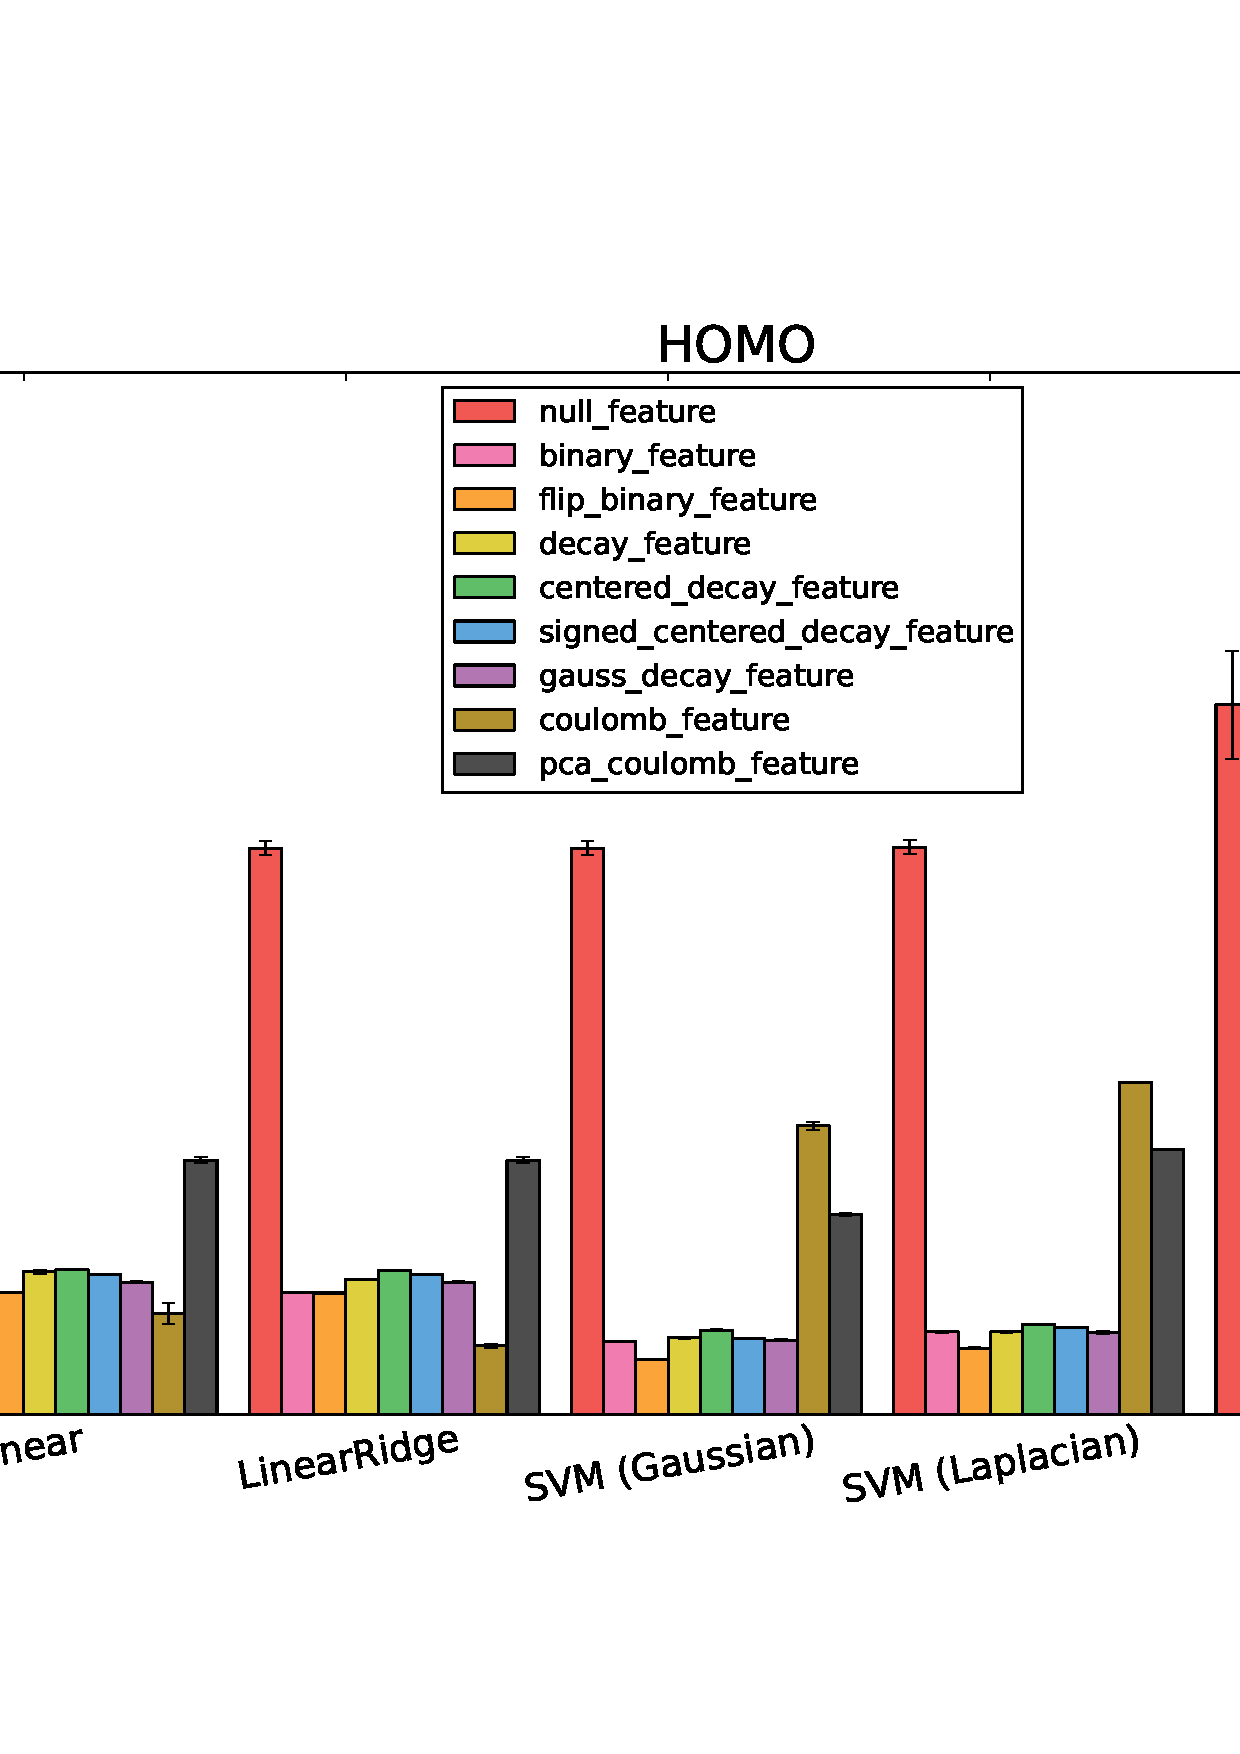
\includegraphics [width=1\textwidth]{homo_results.png}
\caption{test errors of HOMO}\label{homo}
\end{center}
\end{figure}

\begin{figure}[H]
\begin{center}
\includegraphics [width=1\textwidth]{lumo_results.png}
\caption{test errors of LUMO}\label{lumo}
\end{center}
\end{figure}

\begin{figure}[H]
\begin{center}
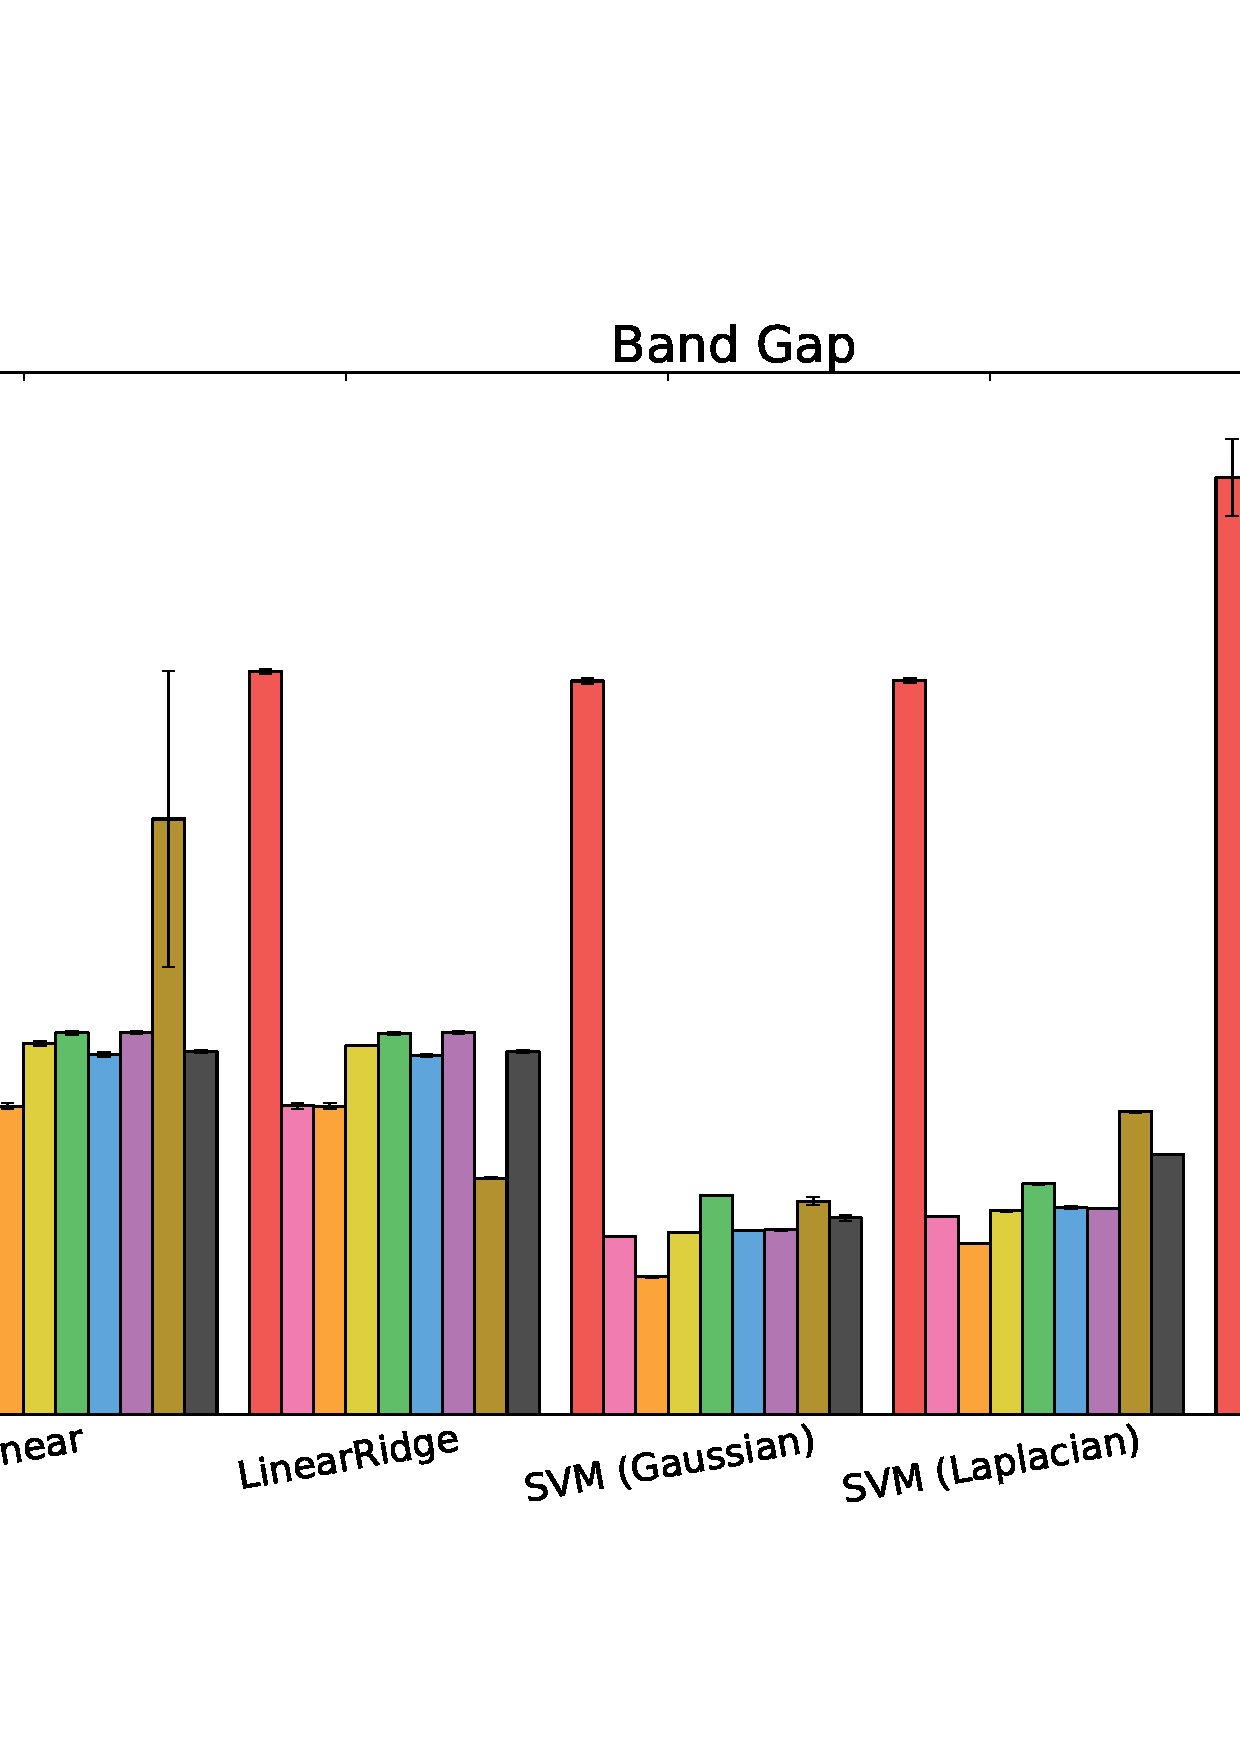
\includegraphics [width=1\textwidth]{gap_results.png}
\caption{test errors of band gap}\label{gap}
\end{center}
\end{figure}
Overall, the flip binary feature vector has the best performance of all the feature vectors. This can be attributed to two factors, 1) it contains more relevant information than the binary feature, so it will quite readily out perform it. 2) This implies that the decay function used in the decay feature vectors is not a good representation of the physical relation between the structures.

To further lower the test errors, we apply Neural Networks with sigmoid or tanh layers to our dataset. Neural Networks' PCA and predictions have shown ideal results in Fig ~\ref{nnpca} and  (Neural INDO comparison plots). Gradient evolution in PCA plots indicates that each layer of the networks can assign the prediction values effectively. 

\begin{figure}[H]
\begin{center}
\includegraphics [width=0.6\textwidth]{07_conn.png}
\caption{Neural Networks PCA}\label{nnpca}
\end{center}
\end{figure}

Neural Networks produce 0.55, 0.60, 0.72 kcal/mol errors for HOMO, LUMO, and Band Gap respectively, which are much lower than the chemical accuracy 1 kcal/mol. 




\section{Conclusion and Future Directions}


We have constructed 1500 polymeric systems and calculated their chemical properties, LUMO, HOMO and band gap, with three different methods. Altogether, there are 12 sets of data or 12000 data points. Based on polymer backbone building blocks and R groups, we have developed 11 different types of feature vectors including a null feature for comparison. Our first goals and milestones are accomplished by effectively implementing machine learning methods on these data sets and producing errors as low as 0.074 eV, 0.076 eV, 0.093 eV for HOMO, LUMO and band gap respectively.

We also achieve our minimum goal by dropping errors down to chemical accuracy (1 kcal/mol (0.047 eV)) through neural networks.

In the future, we should optimize our neural network testing methods to select the best hyperparameters, including layers and nodes. It's necessary to devise corresponding parallelization of codes to fulfill the testing requirements. We should also include more atom types and generalize our methods to nonpolymeric systems.   



\bibliography{final}
\end{document}  
